\documentclass[a4]{article}

\usepackage[left=3cm,right=3cm,top=2cm,bottom=2cm]{geometry} 

\usepackage[utf8]{inputenc}   % otra alternativa para los caracteres acentuados y la "ñ"
\usepackage[           spanish % para poder usar el español
                      ,es-tabla % para los captions de las tablas
                       ]{babel}   
%\decimalpoint %para usar el punto decimal en vez de coma para los números con decimales

\usepackage[T1]{fontenc}
\usepackage{lmodern}

\usepackage{parskip}
\usepackage{xcolor}

\usepackage{caption}
\usepackage{hyperref}
\usepackage{enumerate} % paquete para poder personalizar fácilmente la apariencia de las listas enumerativas
\usepackage{listings}
\usepackage{xcolor}
\usepackage{amsmath}
\definecolor{codegreen}{rgb}{0,0.6,0}
\definecolor{codegray}{rgb}{0.2,0.2,0.2}
\definecolor{codepurple}{rgb}{0.58,0,0.82}
\definecolor{backcolour}{rgb}{0.95,0.95,0.92}

\lstdefinestyle{mystyle}{
	backgroundcolor=\color{backcolour},   
	commentstyle=\color{codegray},
	keywordstyle=\color{codegreen},
	numberstyle=\tiny\color{blue},
	stringstyle=\color{red},
	basicstyle=\ttfamily\normalsize,
	breakatwhitespace=false,         
	breaklines=true,                 
	captionpos=b,                    
	keepspaces=true,                 
	numbers=left,                    
	numbersep=5pt,                  
	showspaces=false,                
	showstringspaces=false,
	showtabs=false,                  
	tabsize=2
}

\lstset{style=mystyle}
\usepackage{graphicx} % figuras
\usepackage{subfigure} % subfiguras

\usepackage{amsfonts}
\usepackage{amsmath}

\definecolor{gris}{RGB}{220,220,220}
	
\usepackage{float} % para controlar la situación de los entornos flotantes

\restylefloat{figure}
\restylefloat{table} 

\newcommand{\HRule}{\rule{\linewidth}{0.5mm}}

\author{Pilar Navarro Ramírez}
\date{\vspace{-5mm}}

\title{\huge APRENDIZAJE AUTOMÁTICO: Práctica 3 \HRule\vspace{-4mm}}

\usepackage[ruled]{algorithm2e}

\begin{document}
\maketitle
\tableofcontents

\newpage

\section{Clasificación: Sensorless Drive Diagnosis}
\subsection{Problema}

En los sistemas de variadores de velocidad electromecánicos los estados defectuosos de los motores síncronos pueden ser detectados en base a medidas de la corriente del motor, sin necesidad de usar sensores adicionales, los cuales son bastante caros para monitorear cada variador de velocidad. Lo que se busca con este dataset es poder predecir el estado de un motor conociendo determinadas medidas de corriente del mismo. 

Partimos de un conjunto de datos con 58509 instancias, donde cada instancia consta de 48 características extraídas de las señales de corriente eléctrica del variador de velocidad. Este puede tener componentes en perfecto estado o defectuosas, lo cual da lugar a 11 estados del motor, cada uno con unas condiciones diferentes. Cada una de estas condiciones ha sido medida varias veces bajo 12 condiciones operativasa distintas, es decir, con diferentes velocidades, carga, fuerzas, etc. 

Nos encontramos, por lo tanto, ante un problema de aprendizaje supervisado, pues disponemos de una muestra etiquetada para el aprendizaje. En concreto se trata de un problema de clasificación multietiqueta, ya que hay 11 clases diferentes en las que queremos clasificar los motores. 

Así pues, tenemos que el espacio de características $\mathcal{X}$ está formado por un conjunto de vectores con 48 valores reales, correspondientes a las distintas medidas de corriente eléctrica del motor. El conjunto de etiquetas $\mathcal{Y}$ consta de 11 clases diferentes, cada una correspondiente a un estado concreto de un motor. La función objetivo $ f $ será la que, dado un vector de características del espacio $\mathcal{X}$, determina la clase a la que pertenecerá el motor al que corresponden esas características, esto es, determina el estado del  motor considerado. 

Tras dividir los conjuntos de datos en training y test (como se explicará en un apartado más adelante), visualizamos los datos del conjunto de entrenamiento para tener una idea de la distribución de los mismos. 
Para ello, necesitamos reducir el número de características, de 48 a 2, para poder ver los datos en 2 dimensiones. Haremos uso de dos técnicas de reducción de la dimensionalidad: PCA (Principal Components Analysis) y t-SNE (t-Distributed Stochastic Neighbouring Entities). 

\textbf{PCA} es una técnica que usa la correlación entre las variables e intenta obtener a partir de ellas (mediante combinaciones lineales de las mismas) el mínimo número de variables posibles que expliquen una cierta variabilidad de los datos originales. Para ello, hace uso de los valores propios más grandes y vectores propios asociados a los mismos, de la matriz de correlaciones, pues estos últimos apuntan en la dirección de mayor variación en el conjunto de datos. Así, se transforma el espacio original de características en otro espacio diferente, intentando explicar la mayor proporción de la varianza de los datos posible. 

Al reducir la dimensionalidad de los datos a 2 con esta técnica obtenemos que la varianza explicada por la primera componente principal es del $19,2\%$ y la explicada por la segunda componente principal es el $13.7\%$. Así, en total se explica el $32.9\%$ de variabilidad, por lo que se pierde bastante información al quedarnos sólo con dos características. 

\textbf{T-SNE}, por su parte, se basa en la distribución de probabilidad de los vecinos alrededor de cada punto. En el espacio de caracterísitas multidimensional original ésta se modela como una distribución normal, mientras que en el nuevo espacio 2D se modela como una distribución t de Student. El objetivo de esta algoritmo es encontrar una proyección en el espacio 2D que minimice la diferencia entre estas dos distribuciones sobre todos los puntos. 

El parámetro principal que controla el ajuste es la perplejidad (\lstinline|perplexity|), que es el número de vecinos más cercanos considerados para hacer coincidir las distribuciones original y ajustada, en cada uno de los puntos. Con un valor bajo de la perplejidad nos centramos más en los puntos cercanos, en la escala local, mientras que un valor alto nos da una visión más general de los datos. Fijamos\\ \lstinline|perplexity=30|, un valor lo suficientemente alto como para tener una visión global de los datos. Valores entre 5 y 50 suelen producir los mejores resultados, como se indica en una de las referencias. 

Este algoritmo es costoso computacionalmente y es recomendable usar otra técnica de reducción de la dimensionalidad antes de aplicarla. Por ello, aplicaremos t-SNE partiendo de los datos obtenidos por PCA (\lstinline|init=x_pca|). 

T-SNE suele proporcionar mejores resultados para la visualización de los datos, de ahí que usemos ambas técnicas. 

Puesto que estas dos técnicas se ven afectada por la escala de los datos, es necesario normalizarlos, para lo cual usamos \lstinline|StandardScaler| de \lstinline|sklearn|. 

Tras visualizar los datos obtenidos por cada una de estas técnicas, haciendo uso de la función \lstinline|plot2D| (la descripción y detalles de implementación de la misma se pueden encontrar en el código), obtenemos las siguientes figuras:

\begin{figure}[H]
	\centering    
	\subfigure[]{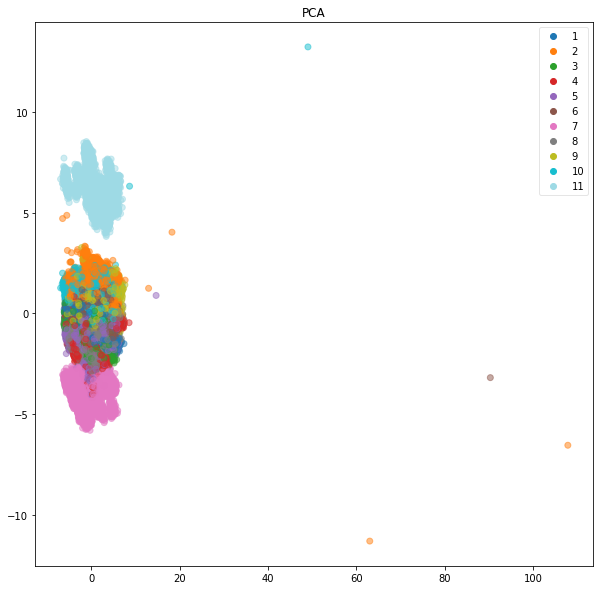
\includegraphics[width=77mm]{img/pca.png}}
	\subfigure[]{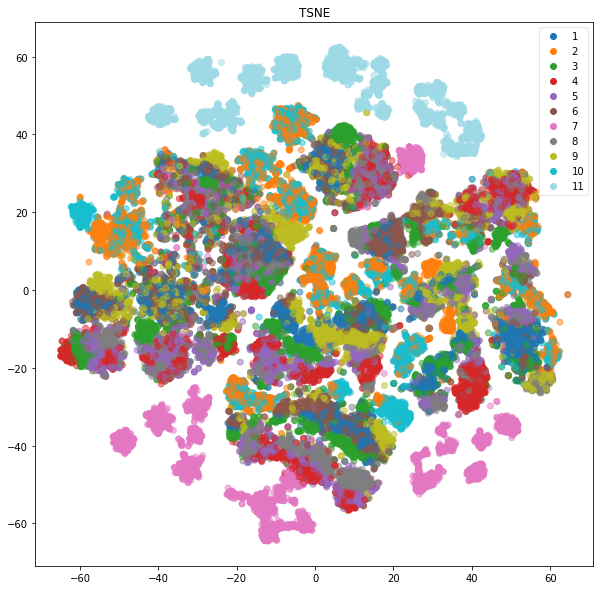
\includegraphics[width=77mm]{img/tsne.png}}
	\caption{}
	\label{fig:dimreduction}
\end{figure}

Nos damos cuenta de que tanto la clase 11 como la 7 están bastante separadas del resto, por lo que los ejemplos pertenecientes a estas clases serán más fáciles de clasificar. Las clases 2 y 10 se superponen entre sí y es probable que se etiquete como clase 2 los ejemplos correspondientes a la clase 10 y viceversa, aunque se diferencian en general del resto de grupos. El resto de las clases se superponen, de modo que será más complicado distinguir entre ellas. 

Cabe notar, además, que hay algunos outliers, hecho que se aprecia mejor en la representación obtenida con PCA, los cuales pueden ser debidos a errores en las medidas de corriente eléctrica

\underline{Referencias:}

 \href{https://towardsdatascience.com/pca-using-python-scikit-learn-e653f8989e60}{https://towardsdatascience.com/pca-using-python-scikit-learn-e653f8989e60}

 \href{https://towardsdatascience.com/visualising-high-dimensional-datasets-using-pca-and-t-sne-in-python-8ef87e7915b}{https://towardsdatascience.com/visualising-high-dimensional-datasets-using-pca-and-t-sne-in-python-8ef87e7915b}
 
 \href{https://www.displayr.com/using-t-sne-to-visualize-data-before-prediction/}{https://www.displayr.com/using-t-sne-to-visualize-data-before-prediction/}
 
\href{https://www.sciencedirect.com/science/article/pii/S1877050920320706}{https://www.sciencedirect.com/science/article/pii/S1877050920320706}

\href{https://scikit-learn.org/stable/auto_examples/preprocessing/plot_scaling_importance.html}{https://scikit-learn.org/stable/auto\_examples/preprocessing/plot\_scaling\_importance.html}
\newpage
\subsection{Selección de la clase de funciones a usar}

La clase de funciones que vamos a usar es la de los polinomios de orden 2, pues permiten obtener un modelo más potente y flexibe que si se usaran sólo características lineales. Sin embargo, la introducción de características cuadráticas aumenta la dimensionalidad, pasando de tener 48 atributos a $48^2=2304$, lo cual hace que el proceso de aprendizaje se vuelva considerablemente lento y costoso. Por lo tanto, será necesario reducir la dimensionalidad, intentando seleccionar sólo las mejores características antes del ajuste de los modelos, como veremos en el apartado de preprocesamiento. Además, al añadir más variables es posible que aumente el número de correlaciones entre las variables del nuevo conjunto o que aparezcan atributos que no aporten información.

Se podrían considerar características polinómicas de mayor orden, pero el entrenamiento se volvería demasiado costoso, por lo que prescindiremos de este tipo de transformaciones. 

La mayor complejidad de la clase de funciones hace que el modelo sea más propenso al sobreajuste, por lo que será conveniente añadir regularización. Este es otro hecho por el cual no consideramos clases más complejas, como polinomios de orden cúbico. 

Para añadir las características cuadráticas usamos la función \lstinline|PolynomialFeatures| de \lstinline|sklearn|, con parámetro 2, para indicar que el grado de las características polinómicas sea 2. Escribimos tambiém \lstinline|include_bias=False|, para que no se añada al vector de caracterísitcas el término de sesgo (constante igual a 1), pues se eliminaría en el preprocesamiento cuando se eliminen las caraterísticas poco informativas. Además, suponemos \lstinline|interaction_only=False|, el valor por defecto, para que se consideren todos los monomios de orden 2. 

La introducción de características cuadráticas es un paso llevado a cabo en el preprocesamiento, por lo que se comentará en ese apartado pero sin mayor explicación, pues ya se han explicado en este punto todos los detalles. 

\underline{Referencias:}

\href{https://scikit-learn.org/stable/modules/generated/sklearn.preprocessing.PolynomialFeatures.html}{https://scikit-learn.org/stable/modules/generated/sklearn.preprocessing.PolynomialFeatures.html}

\subsection{Hipótesis finales}

Se llevará a cabo el mismo \textbf{preprocesamiento} de los datos de entrenamiento (y los de test) para los dos modelos que vamos a estudiar, que consistirá básicamente en la normalización de los datos para que todos tengan media 0 y varianza 1, supresión de observaciones anómalas, eliminación de características que aporten poca información al atributo objetivo, y adicción de característics cuadráticas. 

Se hará uso de la \textbf{regularización} de tipo Ridge, para paliar el sobreajuste. 

Los dos modelos que se estudiarán serán:
\begin{itemize}
 \item \underline{Support Vector Machines} versión Soft con Kernel Linear y técnica de one-vs-rest para la clasificación multietiqueta
\item \underline{Regresión Logística} con one-vs-rest para la clasificación multietiqueta
\end{itemize}


\subsection{Conjuntos de training y test}

El conjunto de datos del que disponemos no está dividido en training y test, por lo que debemos partirlo nosotros. Para ello, puesto que disponemos de más de 10000 instanciass, seguimos la regla general de considerar el 80\% del conjunto de datos para el entrenamiento y el 20\% para test. Las instancias se distribuyen de manera aleatoria en cada uno de los subconjuntos y de manera estratificada, es decir, de forma que haya el mismo número de instancias de cada clase tanto en training como en test.  Así, nos aseguramos de que la muestra de entrenamiento no está sesgada y tanto los datos de training como los de test pertenecen a la misma distribución.

Cabe notar que las clases son balanceadas, esto es, hay exactamente el mismo número de instancias pertenecientes a cada clase en nuestro conjunto de datos, de ahí el hecho de que al dividir los datos en training y test deba seguir habiendo el mismo número de instancias de cada clase. 

Si vemos el número de instancias de cada clase antes de partir el dataset, obtenemos: 

\begin{lstlisting}
	Numero de ejemplos de cada clase:
	Counter({1.0: 5319, 2.0: 5319, 3.0: 5319, 4.0: 5319, 5.0: 5319, 6.0: 5319, 7.0: 5319, 8.0: 5319, 9.0: 5319, 10.0: 5319, 11.0: 5319})
\end{lstlisting}

Así, hay 5319 instancias de cada clase.

Tras dividirlo tenemos:

\begin{lstlisting}
	Numero de ejemplos en cada clase de training:
	Counter({6.0: 4256, 3.0: 4256, 4.0: 4255, 2.0: 4255, 5.0: 4255, 11.0: 4255, 1.0: 4255, 10.0: 4255, 9.0: 4255, 7.0: 4255, 8.0: 4255})
	Numero de ejemplos en cada clase de test:
	Counter({1.0: 1064, 5.0: 1064, 2.0: 1064, 4.0: 1064, 9.0: 1064, 7.0: 1064, 11.0: 1064, 8.0: 1064, 10.0: 1064, 3.0: 1063, 6.0: 1063})
\end{lstlisting}

Observamos que se siguen manteniendo las clases balanceadas en ambos subconjuntos. 

El conjunto de test no volveremos a usarlo hasta la evaluación final, cuando hayamos elegido la hipótesis definitiva. Nos aseguramos así de no contaminar estos datos. 

No obtenemos un conjunto de validación a parte, ya que usaremos validación cruzada como mecanismo para la elección del mejor modelo. 

\subsection{Preprocesamiento}

Puesto que los modelos considerados (SVM y regresión logística) trabajan con características numéricas y los atributos de nuestro dataset son valores reales, no es necesario realizar ninguna codificación de los mismos. 


\textbf{Nota:} En todas las funciones que aparece \lstinline|random_state| como parámetro es porque hay alguna componente aleatoria en el algoritmo, y el parámetro se usa para fijar una semilla. 

\subsubsection{Normalización}
Otro paso importante del preprocesamiento es la normalización de los datos. Puesto que SVM usa las distancias de los puntos al hiperplano separador, es necesario que los datos estén normalizados para que la solución sea correcta, pues en caso contrario unas características tendrían más peso que otras en función de su escala, lo cual no es deseable. Por su parte, Logistic Regression no necesita que los datos estén normalizados pero, como aplicaremos regularización, también será necesario que los datos tengan la misma escala. De otro modo unas características se verían más afectadas por la regularización que otras. Además, la normalización acelera la convergencia. 

Para normalizar lo que haremos será transformar los datos para que tengan media 0 y varianza 1, de la siguiente forma:

$$z=\frac{x-\mu}{\sigma}$$

donde $x$ es el dato a transformar, $\mu$ es la media de los valores de todos los datos para un atributo y $\sigma$ la desviación típica. 

La función \lstinline|StandardScaler| de \lstinline|sklearn.preprocessing| se encarga de hacer esto, siempre que los parámetros \lstinline|with_mean| (para centrar o no los datos en su media) y \lstinline|with_std|
(para que los datos tengan varianza 1) estén a \lstinline|True|, que es el valor por defecto.

\underline{Referencias}:

\href{https://scikit-learn.org/stable/modules/generated/sklearn.preprocessing.StandardScaler.html}{https://scikit-learn.org/stable/modules/generated/sklearn.preprocessing.StandardScaler.html}

\href{https://neerajkumar.org/writings/svm/}{https://neerajkumar.org/writings/svm/}

\href{https://scikit-learn.org/stable/modules/preprocessing.html#preprocessing-scaler}{https://scikit-learn.org/stable/modules/preprocessing.html} 

\subsubsection{Tratamiento de los outliers}
Tras la normalización, intentamos deshacernos de los datos anómalos (outliers), pues ya vimos en la Figura 1 que aparecen algunos en nuestro dataset y estos alteran significativamente la escala de las varibles, además de dificultar el proceso de aprendizaje. Usaremos el algoritmo de Local Outlier Factor (LOF) implementado en la librería de \lstinline|sklearn|. Se trata de un algoritmo de aprendizaje automático semi-supervisado que calcula la desviación de la densidad local de cada punto con respecto a sus vecinos, y considera como outliers los ejemplos que tienen, con diferencia, una menor densidad que sus vecinos. La densidad local se obtiene de los k vecinos más cercanos, parámetro que hay que tunear. El valor del LOF de una observación es igual al ratio de la media de la densidad local de sus k vecinos más cercanos y su propia densidad local. Es esperable que una instancia normal tenga una densidad local similar a sus vecinos, mientras que para una observación anómala se espera que tenga mucha menor densidad local. Así, el ratio será mayor para los puntos anómalos. 

Notamos que, puesto que este algoritmo necesita calcular la distancia de un punto a los demás, es necesario que los datos estén normalizados antes de aplicarlo sobre los mismos. 

El algoritmo LOF sólo se encarga de detectar los outliers, no los elimina, etiquetando con -1 los ejemplos que son considerados anómalos y con 1 los que no. Para deshacernos de ellos será necesario recorrer el resultado proporcionado por este algoritmo, y guardar los índices correspodientes a las instancias que tengan etiqueta -1. Esto es lo que hace la función \lstinline|detectOutliers|, la cual devuelve un vector con las posiciones de los outliers en el datset que se le pasa como parámetro. Posteriormente, eliminamos los ejemplos anómalos de nuestro conjunto de entrenamiento, con la función \lstinline|removeExamples|, tanto en la matriz de características como en el vector de etiquetas. 

Entre los principales parámetros del algoritmo LOF se encuentran el número de vecinos a considerar, $ k $. Según la documentación de la librería scikit-learn, un valor de 20 vecinos suele funcionar bien en general, por lo que seguimos la recomendación y establecemos \lstinline|n_neighbors=20|. Otro parámetro a considerar es la 'contaminación' del dataset, es decir, la proporción de outliers en el conjunto, que puede variar entre $ [0,0.5] $. Puesto que esto es algo que no sabemos a priori, consideramos \lstinline|contamination='auto'|, y se calculará siguiendo la técnica propuesta en el paper original de este algoritmo. Establecemos también \lstinline|algorithm='auto'|, que es el valor por defecto, de manera que se seleccionará como algoritmo para calcular los vecinos más cercanos el que mejor se adapte a nuestro dataset. Para computar la distancia entre los puntos se usará la distancia euclídea, \lstinline|metric='minkowski'| y \lstinline|p=2|, que es la métrica por defecto. Dejamos el parámetro \lstinline|novelty=False|, para indicar que los datos donde queremos detectar los outliers son los de entrenamiento, no buscamos detectar si un nuevo ejemplo es un outlier o no. 

\underline{Referencias:}
\href{https://www.dbs.ifi.lmu.de/Publikationen/Papers/LOF.pdf}{https://www.dbs.ifi.lmu.de/Publikationen/Papers/LOF.pdf}

\href{https://scikit-learn.org/stable/auto_examples/neighbors/plot_lof_outlier_detection.html}{https://scikit-learn.org/stable/auto\_examples/neighbors/plot\_lof\_outlier\_detection.html}

\href{https://scikit-learn.org/stable/modules/outlier_detection.html#id1}{https://scikit-learn.org/stable/modules/outlier\_detection.html}

\href{https://scikit-learn.org/stable/modules/generated/sklearn.neighbors.LocalOutlierFactor.html}{https://scikit-learn.org/stable/modules/generated/sklearn.neighbors.LocalOutlierFactor.html}

\subsubsection{Eliminación de características no informativas}

Es probable que algunas de las características del conjunto de datos no aporten información al atributo objetivo, por lo que es importante detectarlas y eliminarlas para reducir la dimensionalidad y acelerar el proceso de apredizaje. Para hacer esto usaremos la información mutua (\textit{Mutual Information, MI}), que determina la dependencia entre dos variables aleatorias. En otras palabras, especifica la cantidad de información que se obtiene de una determinada variable observando la otra. 

Los métodos basados en información mutua pueden detectar cualquier tipo de dependencia estadística entre dos variables, y no sólo linear. 

Así, usaremos la información mutua para determinar la dependencia entre cada una de las variables del dataset y el atributo objetivo, de modo que, cuanto menor sea esta dependencia, menos informativas serán las variables. 

Cabe notar que se trata de un método univariante, es decir, sólo determina la dependencia con el atributo objetivo de cada variable por separado, por lo que puede haber información que aporten dos o más variabes juntas al atributo objetivo y que no se esté teniendo en cuenta.

La función \lstinline|mutual_info_classif| de \lstinline|sklearn| se encarga de determinar el valor de MI entre dos variables, de manera que será 0 si las variables son independientes y será mayor cuanto más dependencia haya entre las variables. 

El valor de MI se estima haciendo uso de los vecinos más cercanos, por lo que el número de vecinos es un parámetro a considerar. Un mayor número de vecinos reduce la varianza de la estimación, pero puede dar lugar a un sesgo. Así, consideramos el valor por defecto \lstinline|n_neighbors=3|, para que la estimación sea insesgada y se reduzca al menos un poco la varianza. 

Otro parámetro de esta función es \lstinline|discrete_features|, para indicar si las variables son discretas. En nuestro caso son todas continuas, de manera que tomamos \lstinline|discrete_features=False|.

Además de estos parámetros, toma la matriz de características y el vector de etiquetas, como era de esperar. Devuelve un vector con el valor de MI estimado para cada variable. 

En nuestro programa consideramos la función \lstinline|dependence|, la cual llama a \lstinline|mutual_info_classif| para determinar los valores de MI de cada característica de nuestro data set con respecto al atributo objetivo y devuelve los índices de las características que tienen un MI mayor que un cierto umbral, valor que se indica como parámetro de nuestra función. A continuación, \lstinline|removeFeatures| se encarga de eliminar las características del dataset cuyo índice no está incluido en el vector devuelto por la función \lstinline|dependence|.


\underline{Referencias:}

\href{https://scikit-learn.org/stable/modules/generated/sklearn.feature_selection.mutual_info_classif.html}{https://scikit-learn.org/stable/modules/generated/sklearn.feature\_selection.mutual\_info\_classif.html}

\href{https://scikit-learn.org/stable/modules/feature_selection.html#univariate-feature-selection}{https://scikit-learn.org/stable/modules/feature\_selection.html}

\href{https://medium.com/@hertan06/which-features-to-use-in-your-model-350630a1e31c}{https://medium.com/@hertan06/which-features-to-use-in-your-model-350630a1e31c}


\subsubsection{Correlación entre las variables}

Otro aspecto a tener en cuenta es la correlación entre los atributos usados para el aprendizaje, pues si dos atributos tienen un grado fuerte de correlación, podríamos prescindir de uno de ellos, ya que la información que aporta uno puede ser obtenida a partir del otro. 

Para ver si las variables están correladas usaremos el coeficiente de correlación de Pearson. Que se define como: 
$$ \rho_{XY}=\frac{Cov(X,Y)}{\sqrt{Var(X)Var(Y)}}$$
para dos variables aleatorias X e Y, que en nuestro caso serán cada pareja de los atributos del dataset. 

El valor de este coeficiente varía entre -1 y 1, siendo 0 si no hay relación lineal entre las variables. Será 1 si hay una correlación positiva perfecta (cuando una variable aumenta, la otra también lo hace en la misma proporción), y -1 si la correlación es negativa (cuando una variable aumenta, la otra disminuye en la misma proporción, y viceversa). Así, cuanto más lejano a 0 es el coeficiente, mayor dependencia lineal hay entre las variables. 

Utilizamos la función \lstinline|corrcoef| de \lstinline|numpy| para calcular estos coeficientes entre cada par de atributos de nuestro conjunto de datos. Esta función recibe una matriz de características con las observaciones de cada una de ellas. Por defecto, asume que cada fila de dicha matriz representa una variable y cada columna es una observación de todas las variables, esto es, nuestra matriz de características traspuesta. El resultado será una matriz simétrica, donde cada casilla $(i,j)$ tiene el valor del coeficiente de correlación de Pearson entre las variables que ocupan las posiciones (columnas) $i$ y $j$ en la matriz de características original. 

Para visualizar la matriz de correlación de los atributos del conjunto de datos obtenido tras el preprocesamiento haremos uso de la función \lstinline|plotMatrix|, que muestra la matriz que se le pasa como parámetro en forma de mapa de calor. A continuación se muestra el resultado: 
\begin{figure}[H]
	\centering
	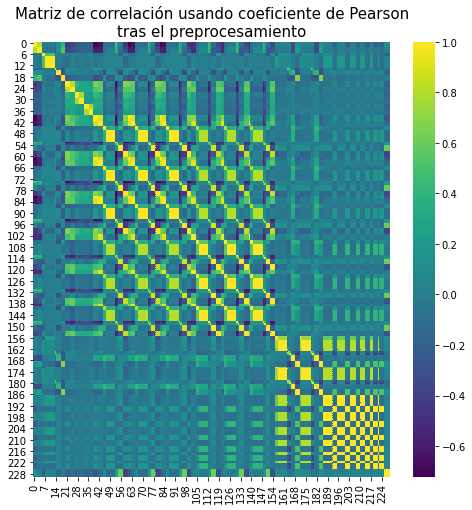
\includegraphics[width=0.6\linewidth]{img/corr}
	\caption{}
	\label{fig:corr}
\end{figure}

Nos damos cuenta de que hay algunas zonas amarillas, correspondientes a variables que tienen una correlación positiva perfecta, y también algunos puntos morados, donde la correlación es negativa. Sin embargo, la mayor parte tiene un color entre azul y verde, de manera que la correlación en general no es muy alta. 

No he visto necesario eliminar variables correladas como parte del preprocesamiento, pues esto será algo de lo que se encargue la regularización durante el entrenamiento de los modelos, en el caso de que sea necesario. 

\underline{Referencias}
\href{https://numpy.org/doc/stable/reference/generated/numpy.corrcoef.html}{https://numpy.org/doc/stable/reference/generated/numpy.corrcoef.html}

\subsubsection{Pasos seguidos}

Enumeramos a continuación los pasos llevados a cabo en el preprocesamiento:

\begin{enumerate}
	\item Normalizamos los datos de entrenamiento y test, ajustando los parámetros usados en la normalización al conjunto de entrenamiento y no al de test
	\item Eliminamos los outliers del conjunto de entrenamiento, tanto de la matriz de características como del vector de etiquetas
	\item Eliminamos los atributos que, en el conjunto de training, aportan poca información al atributo objetivo, en concreto nos quedamos sólo con aquellos que tienen un valor de MI mayor a $ 0.1 $, pues si su valor de MI es $<0.1$ serán prácticamente independientes del atributo objetivo.
	\item Añadimos características cuadráticas, tanto al conjunto de entrenamiento como al de test, pero siempre ajustándose a los datos de entrenamiento y no a los de test. 
	\item Volvemos a normalizar todos los datos, para que las nuevas características introducidas tengan la misma distribución que las demás y para amortizar el efecto que los outliers pudieron tener en la normalización llevada a cabo antes de ser eliminados. 
	\item Eliminamos de nuevo atributos poco informativos, en este caso los que tengan un valor de MI menor que $ 0.2 $, pues es posible que algunas de las nuevas características introducidas no aporten información. Consideramos aquí un umbral superior al introducido en el paso 3., pues allí estamos tratando las características originales, y no las añadidas, de manera que es conveniente mantener el mayor número posible para no perder demasiada información. Sin embargo, al añadir las características cuadráticas, aumenta mucho la dimensionalidad y, en consecuencia, se vuelve muy lento el aprendizaje, por lo que conviene eliminar todas las posibles sin perder mucha información. 
	  
\end{enumerate}

Tras llevar a cabo todos estos pasos, terminamos con un número de características de 230, un cantidad bastante manejable, de manera que hemos ampliado la dimensionalidad original al añadir las características cruadráticas, pero no de manera excesiva, gracias a la eliminación de los atributos poco informativos. 

Al quitar los datos anómalos, el número de instancias del conjunto de entrenamiento pasa a ser 46051. Hemos perdido algunos ejemplos, pero a cambio nos desahecemos de observaciones probablemente anómalas que empeorarían el ajuste más que ayudarlo. 

\subsubsection{Visualización de los datos preprocesados}

Para tener una idea visual del efecto del preprocesamiento, vamos a intentar visualizar los datos preprocesados, haciendo uso de las ténicas de PCA y t-SNE, exactamente de la misma forma que llevabamos a cabo para visualizar los datos originales. Los resultados obtenidos han sido los siguientes: 

\begin{figure}[H]
	\centering    
	\subfigure[]{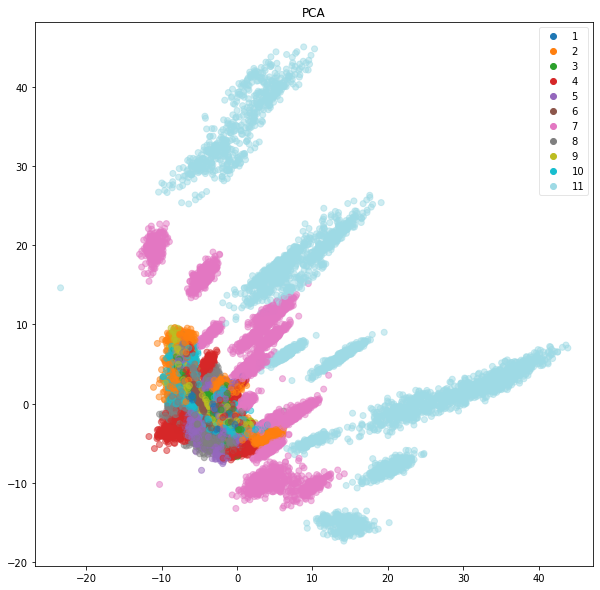
\includegraphics[width=77mm]{img/pca2.png}}
	\subfigure[]{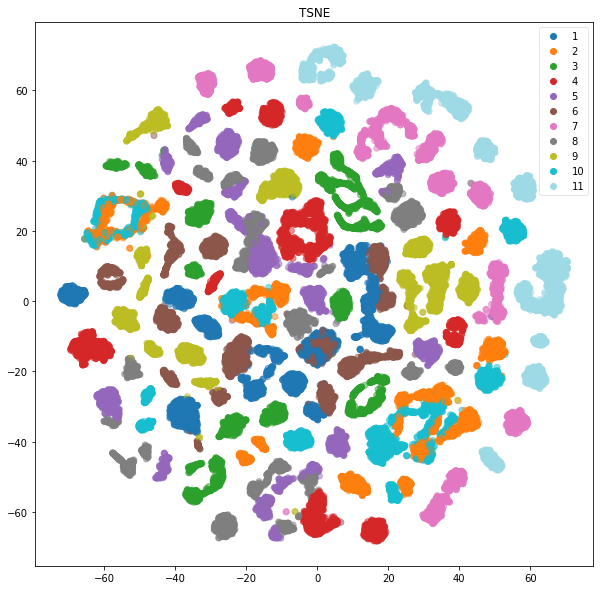
\includegraphics[width=77mm]{img/tsne2.png}}
	\caption{}
	\label{fig:dimreduction}
\end{figure}

Podemos ver que se ha reducido la cantidad de outliers, y que ahora las clases se superponen menos, de manera que las nubes de puntos correspondientes a distintas clases se distinguen con mayor facilidad, lo cual favorecerá al proceso de aprendizaje.

Las clases 7 y 11 siguen siendo separables del resto, mientras que las clases 2 y 10 se siguen superponiendo, aunque algo menos que en los datos originales.

\subsection{Métrica de error}

La métrica que usaremos para medir el error será la precisión, o \textit{accuracy}, que mide la proporción de puntos bien clasificados, proporcionando así valores entre 0 y 1. Puesto que el número de instancias pertenecientes a cada una de nuestras clases está balanceado, esta métrica es adecuada, y se utiliza con frecuencia para determinar la calidad de los modelos en los problemas de clasificación multietiqueta. Además, es simple y fácil de interpretar. 

Por otra parte, visualizaremos también la matriz de confusión, haciendo uso de la función \lstinline|plotMatrix|, para ver los resultados de manera gráfica.  Se trata de una matriz cuadrada de orden igual al número de clases, en la que la casilla $(i,j)$ contiene el número de instancias de la clase $i$ a los que el modelo ha asignado la clase $j$.  Así, el modelo será mejor cuanto mayores sean los valores en la diagonal y menores los valores fuera de esta, pues en la casilla $(i,i)$ se encuentra el número de ejemplos clasificados correctamente y en la $(i,j)$, con $i\neq j$, los ejemplos incorrectamente clasificados. 

Cabe notar que el \textit{accuracy} se calcula sumando los valores de la diagonal de la matriz de confusión, que será el número de instancias bien clasificadas, y dividiendo el resultado entre el número total de ejemplos. 

\subsection{Parámetros y regularización}

Los métodos que vamos a usar para buscar la mejor solución son Regresión Logística y Support Vector Machines con kernel lineal. Descartamos desde un principio el algoritmo Perceptrón, pues no sabemos a priori si los datos son linealmente separables. De hecho esto es muy poco común, por lo que en general la solución que nos dé el Perceptrón no será demasiado buena y mucho menos la óptima. 

\subsubsection{Regresión Logística}

Regresión Logística es un método que asigna a cada muestra la probabilidad de que pertenezca a una clase determinada. Así, para cada muestra, se elije la clase que tenga una probabbilidad más alta. 
 
Esto se consigue mediante la función sigmoide
 $$\sigma(z)=\frac{1}{1-e^{-z}}$$ 
  que devuelve valores en $[0,1]$. 

Lo que se busca es maximizar la verosimilitud de la muestra, es decir, la probabilidad de asignar a cada elemento de la muestra su verdadera etiqueta. Equivalentemente, se intenta minimizar el error, que, en el caso de dos etiquetas es:
$$E_{in}(w)=\frac{1}{N}\sum_{i=1}^{N}\log(1+e^{-y_iw^Tx_i})$$
donde $x_i$ es el punto i-ésimo de la muestra, $y_i$ es su etiqueta (+1 o -1), $ N $ es el tamaño de la muestra y $ w $ es el vector de pesos que determina una función lineal.
El gradiente de este error en un punto $(x,y)$ es $-yx\sigma(-yw^Tx)$.

Para el caso multietiqueta, que es el que nos ocupa, elegimos la aproximación one-vs-rest. Esta consiste en dividir el problema de clasificación multietiqueta en varios problemas de clasificación binaria, considerando los ejemplos de una determinada clase con etiqueta +1 y los ejemplos de todas las otras clases con etiqueta -1 (o al contrario). Así, se entrena un clasificador de regresión logística para cada uno de los subproblemas. Habrá que entrenar, por lo tanto, en total tantos clasificadores como clases haya (en nuestro caso 11), lo cual hace que se vuelva más lento el aprendizaje. Al final, se asocia a cada ejemplo la clase con la mayor probabilidad. 

Otra opción sería la regresión logística multinomial (la otra alternativa que ofrece \lstinline|sklearn| para clasificación multietiqueta con regresión logística), la cual hace uso de la función softmax en lugar de la función sigmoide. Sin embargo, como se describe en el \href{https://medium.com/@jjw92abhi/is-logistic-regression-a-good-multi-class-classifier-ad20fecf1309}{siguiente artículo}, con la función softmax se pueden alterar las proporciones entre pequeñas diferencias, de manera que se introduce un sesgo a favor de una clase en particular, y esto no es deseable. Así, es recomendable usar one-vs-rest frente a regresión logística multinomial para la clasificación multietiqueta. Además one-vs-rest es más fácil de interpretar. 

Hemos seleccionado Regresión Logística por ser un modelo lineal sencillo, que no requiere mucha pontencia de cómputo, fácil de interpretar, eficiente y que proporciona buenos resultados, en general,  en conjuntos de datos no demasiado complejos (como es nuestro caso). Además, no asume ningún tipo de distribución concreta en los datos, la cual será desconocida en la mayoría de los casos. 

Por otra parte, se ha demostrado experimentalmente (según lo comentado en clase de teoría) que en los casos con bastante ruido la maximización de la verosimilitud en la muestra da lugar a mejores soluciones que la optimización por separabilidad, como es el caso de SVM. Además, proporciona mejores resultados que SVM-soft, por ejemplo, en el caso en que las clases se superponen. Estos dos fenómenos se dan en nuestro dataset, como vimos en las Figuras 1 y 3.

En cuanto a los algoritmos para resolver el problema de optimización (minimizar $E_{in}(w)$), \lstinline|sklearn| ofrece varias opciones, que describimos brevemente a continuación: 
\begin{itemize}
	\item \textbf{newton-cg} es el método de Newton, que usa la matriz Hessiana de la función a minimizar en lugar del gradiente, como sigue: $$ w_{k+1}=w_{k}-H^{-1}\nabla f(w_k)$$ 
	donde $w_{k}$ son las coordenadas obtenidas en la k-ésima iteración del algoritmo, $f$ es la función a minimizar y $H$ es la matriz Hessiana de la misma
	\item \textbf{lbfgs} (Limited-memory Broyden–Fletcher–Goldfarb–Shanno). Es una modificación del método de Newton, donde la matrix Hessiana se aproxima usando actualizaciones especificadas por evaluaciones del gradiente, es decir, se usa una estimación de la inversa de la matriz Hessiana. 
	\item \textbf{sag}(Stochastic Average Gradient), variación del gradiente descendente estocástico, que usa datos de las iteraciones anteriores para intentar que la convergencia sea más rápida. 
	\item \textbf{saga}, una variante de sag que también admite regularización L1. 
	\item \textbf{liblinear}. Este es el método que usaremos, por lo que se explica a continución en más detalle. 
	Se basa en el algoritmo de descenso coordinado (CD), un algoritmo de optimización que, en cada iteración,  realiza una búsqueda unidimensional a lo largo de una dirección de coordenadas (en nuestro caso una coordenada se corresponde con una característica del dataset), elegida por una cierta regla de selección, e intenta minimizar sobre el hiperplano correspondiente a esa coordenada, manteniendo fijas todas las otras coordenadas. Así, se resuelven varios problemas de optimización univariantes en vez de un único problema multivariante. 
	
	Para elegir la coordenada, lo más común es iterar cíclicamente sobre todas las direcciones, una cada vez, minimizando la función objetivo con respecto a esa coordenada en cada iteración. 
	
	El pseudocódigo de este algoritmo quedaría como sigue: 
		
	\begin{algorithm}
	\DontPrintSemicolon
	\caption{\sc coordinate descent}
	\Begin{
		k $\leftarrow$ 0 \\
		$ w^0 $ $\leftarrow$ punto inicial\\
		\Repeat{max\_num\_iteraciones}{
			Elegir $i_k$ \textbf{in} $\{1,...,n\} $  \tcp*{n es el numero de caracteristicas}	
			$ w^{k+1}_{i_k} $ $\leftarrow$ $w^k_{i_k}- \alpha \left[\nabla f(w^k)_{i_k}\right]$
		} 
	}
	\end{algorithm}	

donde $f$ es la función que se desea minimizar (en nuestro caso es el $E_{in}$), $ \left[\nabla f(w^k)_{i_k}\right] $ es la componente $i_k$-ésima del gradiente de dicha función evaluado en el vector de pesos, y $\alpha$ es la tasa de aprendizaje. 
\end{itemize}
Hacemos uso de \lstinline|LogisticRegression| de \lstinline|sklearn|. Analizamos a continuación cada uno de los parámetros de este modelo.

\begin{itemize}
	\item \lstinline|penalty| sirve para especificar el tipo de regularización a usar. Establecemos  \lstinline|penalty='l2'|, para usar regularización de tipo L2, que explicaremos más adelante.
	\item \lstinline|dual| para indicar si se usa la formulación dual o primal del problema de optimización. Puesto que tenemos más ejemplos que características, usaremos la formulación primal, es decir, dejamos \lstinline|dual=False|
	\item En \lstinline|tol| especificamos la tolerancia que deseamos que se considere como criterio de parada. Dejamos el valor por defecto, \lstinline|tol=0.0001|, ya que si lo disminuimos para conseguir una mejor solución se necesitarían muchas más iteraciones para alcanzar esa tolerancia y aumentaría el tiempo de cómputo. 
	\item \lstinline|C| es el parámetro que especifica el efecto de la regularización, de manera que valores mayores conllevan un menor efecto de la regularización y valores más pequeños indican una regularización más fuerte. 
	\item \lstinline|fit_intercept| lo ponemos a True (valor por defecto), para que se añada un término de sesgo, con \lstinline|intercept_scaling=1| (valor por defecto), para que el valor del sesgo sea la constante igual a 1.
	\item \lstinline|class_weight| lo dejamos a None porque nuestras clases son balanceadas y consideramos el mismo peso para todas ellas. 
	\item \lstinline|solver| es el algoritmo usado para resolver el problema de optimización, que ya hemos explicado.
	\item \lstinline|max_iter| como su nombre indica es el máximo número de iteraciones del 'solver'. Consideramos \lstinline|max_iter=1000| para que tenga suficientes iteraciones para converger pero no necesite demasiado tiempo de cómputo. 
	\item Establecemos \lstinline|multi_class='ovr'|, para que se use la técnica de one-vs-rest en la clasificación multietiqueta, por los motivos ya explicados.
	\item Dejamos \lstinline|warm_start=False|, pues según la documentación de sklearn es inútil si el solver considerado es liblinear, como es nuestro caso. 
	\item \lstinline|n_jobs| también se ignora si el solver es liblinear. Sirve para indicar el número de núcleos a usar en la paralelización en el cado de múltiples clases, con \lstinline|multi_class='ovr'|
	\item 	\lstinline|l1_ratio| lo ignoramos, porque no vamos a usar regularización de tipo elastic-net. 
	\item  \lstinline|random_state| se usa con los \textit{solvers} sag, saga y liblinear (el que seleccionamos nosotros) para fijar la semilla a la hora de barajar los datos. 
\end{itemize}

Así, los parámetros que tenemos que configurar para este algoritmo son la constante de regularización \textbf{C} y el tipo de \textbf{solver} a usar. Para buscar los mejores valores consideramos un grid de parámetros, haciendo uso del objeto \lstinline|GridSearchCV| de sklearn, que lleva a cabo una búsqueda exhaustiva sobre los parámetros que se le especifican, determinando cuales son los mejores por medio de validación cruzada (mecanismo que explicaremos más adelante).

Entre los parámetros que toma \lstinline|GridSearchCV| están el modelo a configurar (\lstinline|estimator|), un diccionario con los parámetros como \textit{keys} y los valores a probar para los mismos (\lstinline|param_grid|), la métrica usada para evaluar el modelo con validación cruzada en el conjunto de validación (\lstinline|scoring='accuracy'| para que se use el accuracy, como ya comentamos en el apartado correspondiente), el número de procesadores a usar para la ejecución en paralelo (\lstinline|n_jobs=-1| para que tome todos los procesadores del ordenador y termine antes), un parámetro para determinar si se reentrena el modelo al final con los mejores valores encontrados (tomamos \lstinline|refit=True|, que es el valor por defecto, para poder obtener después el error de validación cruzada del mejor estimador) y el número de particiones usadas en validación cruzada (consideramos \lstinline|cv=5|, que es la reglar general). El resto de parámetros no tienen influencia en la búsqueda, por lo que no los consideramos. 

Para la constante de regularización consideramos 11 valores entre $10^{-5}$ y  $10^{5}$, esto es, 0.000001, 0.00001,0.0001,.....,10000,100000. Así, podemos determinar si la regularización debe o no afectar demasiado para obtener una buena solución. 

Para el \textit{solver} tomamos todas las opciones que nos da \lstinline|sklearn|, ya explicadas, para determinar cuál de ellos ofrece una mejor solución. 

Tras llevar a cabo la búsqueda, los mejores parámetros encontrados fueron \lstinline|solver=liblinear| (de ahí que usemos este algoritmo para la optimizaión) y $ C=100000 $ (el máximo valor de los proporcionados, resultado que analizaremos más adelante).

\textbf{Nota:} La configuración de parámetros lleva bastante tiempo, en mi ordenador tardó casi un día, por lo que no es recomendable su ejecución nuevamente, a no ser que sea estrictamente necesario. Por ese motivo considero la variable \lstinline|TUNING|, que determina si se ejecuta o no dicha configuración. En el script entregado se establece a \textbf{False}. 

\underline{Referencias:}

\href{https://www.geeksforgeeks.org/advantages-and-disadvantages-of-logistic-regression/}{https://www.geeksforgeeks.org/advantages-and-disadvantages-of-logistic-regression/}

\href{https://stackoverflow.com/questions/38640109/logistic-regression-python-solvers-defintions/52388406}{https://stackoverflow.com/questions/38640109/logistic-regression-python-solvers-defintions/52388406}

\href{https://en.wikipedia.org/wiki/Coordinate_descent}{https://en.wikipedia.org/wiki/Coordinate\_descent}

\href{http://www.optimization-online.org/DB_FILE/2014/12/4679.pdf}{http://www.optimization-online.org/DB\_FILE/2014/12/4679.pdf}

\href{https://scikit-learn.org/stable/modules/generated/sklearn.linear_model.LogisticRegression.html}{https://scikit-learn.org/stable/modules/generated/sklearn.linear\_model.LogisticRegression.html}

\href{https://scikit-learn.org/stable/modules/generated/sklearn.model_selection.GridSearchCV.html}{https://scikit-learn.org/stable/modules/generated/sklearn.model\_selection.GridSearchCV.html}

\subsubsection{Regularización}

Como hemos aumentado la complejidad de nuestra clase de funciones, seleccionando características cuadráticas, la varianza de la clase de funciones también ha incrementado, y en consecuencia aumenta el ruido determinista, siendo el sobreajuste más probable. Por lo tanto, es importante incluir algún tipo de regularización, esto es, restricciones a las funciones de la clase que se pueden elegir (en concreto a los pesos que determinan a las mismas).

En \lstinline|LogisticRegression| de \lstinline|sklearn| los tipos de regularización permitida son L1 (regularización de tipo Lasso), L2 (regularización de tipo Ridge) y Elastic-Net (una mezcla de ambos). El primer tipo es útil cuando hay muchas características en el dataset, algunas de las cuales no aportan información y no son importantes para el aprendizaje. Puesto que en el preprocesamiento hemos eliminado características que no aportaban información, a priori la regularización L1 no ayudará demasiado, porque hemos hecho su trabajo antes del aprendizaje. Así pues, vamos a considerar la regularización de tipo L2, pues esta ayuda en el caso en que las variables estén correlacionadas, incentivando a los pesos asociados a las características que se pueden obtener a partir de otras a tomar valores bajos. Como vimos en la matriz de correlaciones entre las características (Figura 2), en nuestro dataset hay algunas características correlacionas, tanto positiva- como negativamete, de modo que la regularización de tipo Ridge ayudará a darle menos importancia a dichas características y a reducir la complejidad de la clase. 

Lo que se busca con la regularización de tipo Ridge es minimizar el error $$ E_{aug}(w)=E_{in}(w)+\lambda \|w\|_2^2$$ donde $\lambda$ es un hiperparámetro que controla el efecto de la regularización. Cuanto mayor sea el valor de $\lambda$ más pequeños serán los pesos y mayor efecto tendrá la regularización.

Derivando este error \textit{aumentado} se obtiene: $$ \nabla_{w_j} E_{aug}(w)=\nabla_{w_j} E_{in}(w)+2\lambda w_j$$.


\subsubsection{Support Vector Machines}

Una máquina de soporte de vectores construye un hiperplano separador en un espacio con alta dimensionalidad, el cual se usa para la clasificación. Este hiperplano se intenta buscar lo más 'grueso' posible, es decir, que maximice la distancia entre los puntos más cercanos de dos clases diferentes, llamados vectores de soporte, pues la dimesión VC es menor cuanto más grueso sea el hiperplano separador (el margen entre dos clases), de manera que el error de generalización también disminuye al aumentar el ancho del margen.   

El enfoque usado será SVM-Soft, es decir, se acepta una cierta violación del margen de separación, $\xi_n$ para cada punto de la muestra $(x_n,y_n)$ . Así, se permite que algunos puntos estén mal clasificados o dentro del margen de separación, de manera que este enfoque es más robusto al ruido y es menos probable que incurra en sobreajuste. 

Idealmente todos los puntos deberían estar bien clasificados y fuera del margen, es decir, cumpliendo que $y_n(w^Tx_n+b)\geq 1$, pero no sabemos si el problema es separable con un hiperplano, por lo que se permite a las muestras estar a una distancia $\xi_n$ de su correspondiente borde del margen. 

Así, dado un conjunto de instancias $x_n\in\mathbb{R}^d, n=1,2,...,N$ (N es el número de muestras de entrenamiento) distribuidas en dos clases y un vector de etiquetas $y\in {-1,1}^N$, se intenta buscar un vector de pesos $w \in \mathbb{R}^d$ para cada instancia y el valor del sesgo $b \in \mathbb{R}$ tales que la predicción proporcionada por $sign(w^Tx_n+b)$ sea correcta para la mayor parte de las muestras posible. La formulación primal del problema de optimización a resolver es como sigue: 
\begin{align*}
\min\limits_{b,w,\xi}\frac{1}{2}w^Tw + C \sum_{n=1}^{N}\xi_n\\
\text{Sujeto a: }  y_n(w^Tx_n + b)\geq 1 - \xi_n, n=1,...,N\\
\xi_n \geq 0 \text{ para } n=1,...,N
\end{align*}

La formulación dual es recomendable cuando el número de características es mayor al número de ejemplos del que se dispone, el cual no es nuestro caso, por lo que usamos el problema primal y no entramos en la descripción del dual. 

Si se usa la función de pérdida \textit{hinge loss}, $e_n(w,b)=max(1-y_n(w^Tx_n+b),0)$ para un punto $(x_n,y_n)$, la formulación primal puede escribirse como

\begin{align*}
\min\limits_{b,w}\frac{1}{2}w^Tw + C \sum_{n=1}^{N}max(1-y_n(w^Tx_n+b),0)
\end{align*}

que es el problema de optimización que resuelve \lstinline|LinearSVC|, modelo que vamos a usar. 

El parámetro $C$ es el peso de la penalización porque un punto quede dentro del margen de separación o esté mal clasficado, o lo que es lo mismo, la inversa de la influencia de la regularización, como ocurría en regresión logística. Por lo tanto, cuanto menor sea el parámetro C más peso tendrá la regularicación y menos la violación del margen determinada por los valores de $\xi_i$.  

Elegimos SVM como segundo modelo porque proporciona la solución óptima, en el sentido de que minimiza la dimensión de VC, en el caso en que los datos sean separables. Si no son separables, lo cual ocurre normalmente, SVM-Soft también encuentra la solución de menor error de generalización para cada valor del parámetro C, lo cual no está garantizado para otros modelos. 

Los parámetros que toma \lstinline|LinearSVC| coinciden en su mayoría con los que considera \lstinline|LogisticRegression|, ya explicados, y establecemos los mismos valores que para regresión logística por los motivos ahí descritos, y para que tenga sentido comparar los resultados de ambos modelos (como el máximo número de iteraciones, la tolerancia, la técnica de clasificación para múltiples clases, etc). 
El único parámetro adicional en este clasificador es la función de pérdida \lstinline|loss|, que puede ser \lstinline|'hinge'| o \lstinline|'squared_hinge'|, siendo esta última el cuadrado de la función de pérdida \lstinline|'hinge'|. Consideramos \lstinline|loss='squared_hinge'|, pues esta función es diferenciable, al contrario que \textit{hinge}, por lo que al usar Coordinate Descent se puede calcular su gradiente sin dificultad. Además, penaliza más los errores grandes, de manera que es más robusto a los outliers que pudieran quedar en nuestro conjunto de entrenamiento.  

Para este modelo, si \lstinline|dual=False|, entonces no hay aleatoriedad y el parámetro \lstinline|random_state| no tiene efecto, por lo que no lo consideramos. 

\lstinline|LinearSVC| también usa como \textit{solver} para resolver el problema de optimización la técnica \textit{liblinear}. 

En este caso el único parámetro a configurar es el valor de C. Repetimos el mismo procedimiento que para Regresión Logística, con \lstinline|GridSearchCV| y con un rango de valores entre $10^{-5}$ y $10^5$, al igual que antes, y volvemos a obtener que el mejor valor es $C=10000$.

\underline{Referencias}:

\href{https://scikit-learn.org/stable/modules/generated/sklearn.svm.LinearSVC.html}{https://scikit-learn.org/stable/modules/generated/sklearn.svm.LinearSVC.html}

\href{https://scikit-learn.org/stable/modules/svm.html#tips-on-practical-use}{https://scikit-learn.org/stable/modules/svm.html}

\href{https://www.machinecurve.com/index.php/2019/10/15/how-to-use-hinge-squared-hinge-loss-with-keras/}{https://www.machinecurve.com/index.php/2019/10/15/how-to-use-hinge-squared-hinge-loss-with-keras/}

\subsubsection{Análisis del parámetro de regularización obtenido}

Intentamos explicar ahora el valor de C obtenido como el mejor por la búsqueda en rejilla, tanto para regresión logística como para SVM. 

C=100000 equivale a un valor de $\lambda$ de $0.000001$, esto es aproximadamente 0. Si hubieramos puesto un rango de parámetros mayor en la búsqueda en rejilla, considerando valores mayores a $10^5$ posiblemente habríamos obtenido el más grande de ellos como el mejor. Esto nos hace pensar que la regularización no está ayudando, pues no tiene influencia y en el caso de restringir aún más los pesos el resultado empeoraría. 

Por lo tanto, es posible que la regularización elegida no sea la adecuada, y, aunque haya algunas variables correlacionadas, no sea suficiente para no tenerlas en cuenta. Quizás la regularización de tipo L1 sí habría ayudado, pues, aunque hayamos eliminado algunas características al principio, es posible que siga habiendo algunas que no sean importantes, o que las eliminadas sí aportaran información, por ejemplo al considararlas en conjunto con otras variables y no de manera aislada. 

Cabe mencionar que, según la documentación de sklearn, valores altos de C aumentan considerablemente el tiempo de cómputo, por lo que el aprendizaje tarda bastante tiempo. Se podría diminuir el valor de este parámetro sin que los resultados empeoren demasiado y que la ejecución sea más rápida. Así, he disminuido un orden el valor de este parámetro para los modelos finales, considerando $C=10000$.

\subsection{Selección de la mejor hipótesis}

Para determinar cuál de las dos hipótesis estudiadas es mejor, usamos el error de validación. En concreto, en vez del error consideramos la bondad del modelo, el accuracy (proporción de ejemplos bien clasificados), como ya comentamos. El error sería simplemente $ 1-accuracy $. Este error es un estimador insesgado para el error fuera de la muestra y es pesimista, por lo que la mejor hipótesis seleccionada tendrá un rendimiento mejor que el proporcionado por $E_{val}$. Así, escogeremos la hipótesis que tenga mayor accuracy en validación o, equivalentemente, que presente el menor error de validación. 

En vez de considerar un sólo conjunto de validación lo que haremos será usar la técnica de validación cruzada con K particiones (K-fold cross-validation), que consiste en dividir el conjunto de entrenamiento en K subconjuntos, entrenar el modelo en K-1 de ellos y evaluarlo en el subconjunto restante. Esto se repite K veces, dejando fuera un subconjunto diferente de validación cada vez, de modo que todos los datos del dataset formen parte tanto de training como de validación. Finalmente se proporciona como error (o accuracy en nuestro caso) la media de los errores de validación obtenidos en cada subconjunto de validación considerado. Así, se tiene que
$$E_{cv}=\frac{1}{K}\sum_{i=1}^{K}E_{val}(g_i^-)$$ donde $g_i^-$ es la mejor hipótesis obtenida con los K-1 subconjuntos de entrenamiento en la iteración i-ésima. 

Hacemos uso de \lstinline|cross_val_score| de la librería \lstinline|sklearn| para obtener el error de validación cruzada de cada uno de nuestros modelos. Los parámetros que consideramos de este método son el clasificador que se quiere evaluar, \lstinline|estimator|, la matriz de características \lstinline|X|, el vector de etiquetas \lstinline|y|, la métrica usada para la evaluación \lstinline|scoring='accuracy'|, el número de particiones (consideramos \lstinline|cv=5| que es la regla general) y \lstinline|n_jobs| que tomamos como -1 para que se usen todos los procesadores del ordenador para la ejecución en paralelo de los entrenamientos y evaluaciones de los K modelos. 

\lstinline|cross_val_score| divide el conjunto de datos en varios subconjuntos de manera estratificada, esto es, manteniendo el mismo número de ejemplos de cada clase en los distintos subconjuntos. Devuelve un vector con los valores de accuracy obtenidos para cada uno de los K subconjuntos, por lo que hacemos la media de todos los valores del vector para obtener $E_{cv}$. 

La función \lstinline|printCV| se encarga de llamar a \lstinline|cross_val_score|, con los parámetros ya especificados, y hacer la media de todos los valores obtenidos. En el caso de que se llame a \lstinline|printCV| justo después de llevar a cabo un GridSearch (parámetro \lstinline|grid=True|) muestra los mejores parámetros obtenidos y el error de validación cruzada del mejor de los estimadores encontrados.

Los valores medios de accuracy de validación cruzada para cada uno de los modelos considerados han sido: 

\begin{lstlisting}
	Support Vector Machines:  0.9824542411465496
	Regresion Logistica:  0.9832142704322158
\end{lstlisting} 

Nos damos cuenta de que ambos modelos proporcionan muy buenos resultados, con una precisión de más del 98\% en media en las 5 particiones consideradas para validación cruzada. Así, podemos decir que las decisiones tomadas tanto en el preprocesamiento como en la elección de los modelos han sido adecuadas. Quizás con otro tipo de regularización los resultados habrían sido mejores, como ya comentamos. Teniendo en cuenta que solo estamos trabajando con modelos lineales y características cuadráticas, esto es, modelos no demasiado potentes y clase de funciones no muy compleja, estos resultados son muy buenos. El hecho de no usar clases complejas puede hacer que haya menos tendencia al overfitting, lo que hace que los modelos generalicen bien fuera de la muestra. 

Aunque los dos modelos ofrecen resultados muy parecidos, regresión logística nos da en este caso un error de validación cruzada ligeramente inferior. Esto puede ser debido al hecho que comentamos de que regresión logística muestra experimentalmente mejores soluciones que SVM en el caso de que las clases se superpongan. Sin embargo, también podría deberse a otros factores como la aleatoriedad en el algoritmo de Coordinate Descent. Es posible que con otra semilla en Regresión Logística, SVM ofrezca una mejor solución. En cualquier caso, teniendo en cuenta el accuracy de validación cruzada, elegimos como mejor modelo Regesión Logística. 

Para calcular los valores de accuracy obtenidos por Regresión Logística en el conjunto de test y en el propio conjunto de entrenamiento implementamos la función \lstinline|printFinalResults|. Si llamamos a esta función con el modelo de Regresión Logística y con los mejores parámetros encontrados, obtenemos lo siguiente:

\begin{lstlisting}
Accuracy en el conjunto de entrenamiento:  0.9858417841089228
Accuracy en el conjunto de test:  0.9788924970090582
\end{lstlisting}

Como era de esperar el accuracy en el conjunto de entrenamiento es más alto que el de validación y el de test, y el del conjunto de test es más bajo. No obstante, la diferencia entre $E_{test}$ y $E_{in}$ es de 0.007, de modo que el modelo generaliza bien fuera de la muestra, como ya hemos dicho. 

$E_{test}$ proporciona una buena estimación para el error fuera de la muestra. De hecho es un estimador insesgado. Por lo tanto, podemos considerar que $E_{out}\approx E_{test}$.

La función \lstinline|printFinalResults| también nos muestra la matriz de confusión sobre el conjunto de test, que es la siguiente: 
\begin{figure}[H]
	\centering
	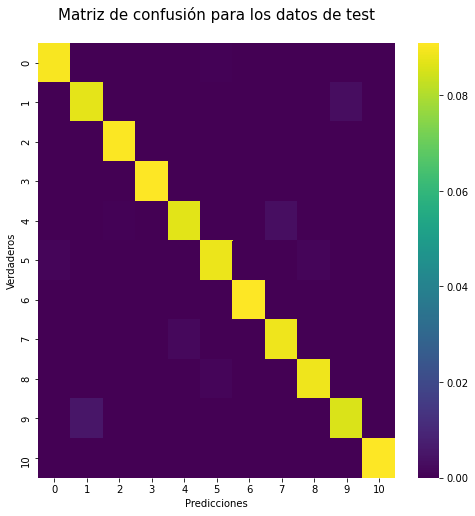
\includegraphics[width=0.5\linewidth]{img/confussion}
	\caption{}
	\label{fig:confussion}
\end{figure}

Esta matriz es prácticamente diagonal, por lo que la mayoría de los ejemplos se clasifican correctamente. Sin embargo, en algunos casos se confunden las instancias pertenecientes a las clases 1 y 9, ó 4 y 7, por lo que estas clases deben presentar características bastante parecidas. 

\underline{Referencias:}

\href{https://scikit-learn.org/stable/modules/generated/sklearn.model_selection.cross_val_score.html}{https://scikit-learn.org/stable/modules/generated/sklearn.model\_selection.cross\_val\_score.html}

\href{https://scikit-learn.org/stable/modules/cross_validation.html#cross-validation}{https://scikit-learn.org/stable/modules/cross\_validation.html}

\subsection{Entrenamiento con todos los datos}

Una vez seleccionada y evaluada la mejor hipótesis podemos utilizar todos los datos de los que disponemos para entrenar el modelo nuevamente y afinar la hipótesis obtenida. 

Para ello unimos los datos de training y test en un único conjunto, y los barajamos para que los datos de test no queden todos al final. A continuación aplicamos el preprocesamiento al nuevo conjunto de datos, tal y como se explicó en el apartado correspondiente. Así, obtenemos un conjunto con 227 características y 57570 instancias. 

Llamamos ahora a la función \lstinline|printCV| con el mejor modelo seleccionado, esto es, Regresión Logística con solver \textit{liblinear} y parámetro $ C=10000 $, y con el nuevo conjunto de datos. Esta función se encargará de llevar a cabo validación cruzada con K=5, como ya hemos explicado. 

Usaremos el error de validación cruzada como estimación para el error fuera de la muestra, ya que ahora no se dispone de un conjunto de test para estimar el mismo. Se cumple que $E_{out}(h)\leq E_{cv}(h)$, siendo h la hipótesis final elegida. Es decir, $E_{cv}$ es una cota pesimista para el error de la mejor hipótesis fuera de la muestra, y podemos usarla para tener una estimación de la bondad del modelo. 

Para nuestro modelo, usando todos los datos para validación cruzada, obtenemos $$E_{cv}= 1-0.9829946152509988=0.01700538474900115
$$

Al entrenar con más datos la solución obtenida mejora, como era de esperar, pues entrenando sólo con el 80\% de los datos obtuvimos un $$E_{out}\approx E_{test}=1-0.9788924970090582=0.021107502990941773 > 0.017
$$

Y sabemos que ahora $E_{out}\leq E_{cv}=0.017 < 0.0211$, por lo que podemos concluir que la hipótesis obtenida entrenando con todos los datos es mejor que la que se obtuvo entrenando solamente con un subconjunto de ellos, de manera que es conveniente usar todos los datos para el entrenamiento una vez seleccionado el mejor modelo.  

\textbf{AVISO!} La ejecución del script para el problema de clasificación (\lstinline|clasificacion.py|) es bastante lenta, en un ordenador con 8 núcleos tardó alrededor de 2 horas y media, debido a que validación cruzada es muy costosa computacionalmente. 

\section{Regresión}


\subsection{Problema}

Los materiales superconductores son aquellos que conducen la corriente con resistencia cero a temperaturas extremadamente bajas. Estos materiales tienen aplicaciones prácticas tanto en el campo de la medicina como de la física. Sin embargo, debido a las bajas temperaturas a las que hay que someter a estos materiales para que tengan resistencia cero, su uso se ha visto reducido. Además, predecir la temperatura crítica a la que que se vuelve cero la resistencia eléctrica ha sido un problema desde que se descubrió la superconductividad. Cabe así preguntarse si será posible predecir dicha temperatura mediante técnicas de aprendizaje automático, partiendo de un conjunto de características basadas en propiedades físicas y químicas de los materiales.

Se dispone de un conjunto de datos, \lstinline|train.csv|, con 21263 ejemplos correspondientes a distintos materiales superconductores, cada uno de los cuales tiene asociado un total de 81 características, tanto físicas como químicas (por ejemplo densidad, masa atómica, afinidad electrónica, punto de fusión, valencia, etc.), así como un valor de la temperatura crítica a la que dicho material alcanza la resistencia cero. 

Deducimos así que estamos ante un problema de aprendizaje supervisado, ya que disponemos de un conjunto de datos con sus correspondientes valores del atributo a predecir. Podemos ver el problema como un problema de regresión lineal, pues el atributo objetivo es un valor real. 

El espacio de características $\mathcal{X}$ está constituido por vectores de valores reales de longitud 81, donde cada posición corresponde a una característica del material en cuestión. El espacio $\mathcal{Y}$
estará formado por todos los valores que puede tomar la temperatura crítica, que es un valor real, por lo que podemos considerar $\mathcal{Y}=\mathbb{R}$. Finalmente, la función objetivo $f$ se encargará de asignar a cada vector de caracteríticas dado del espacio $\mathcal{X}$ un valor de la temperatura crítica. 

Visualizamos los datos de entrenamiento, una vez hecha la división del conjunto de datos en training y test, haciendo uso de la función \lstinline|plot2D|. Para ello debemos reducir antes la dimensionalidad a dos componentes, para lo cual haremos uso de PCA y T-SNE exactamente de la misma forma que en el problema de clasificación. Los gráficos obtenidos han sido los siguientes: 

\begin{figure}[H]
	\centering    
	\subfigure[]{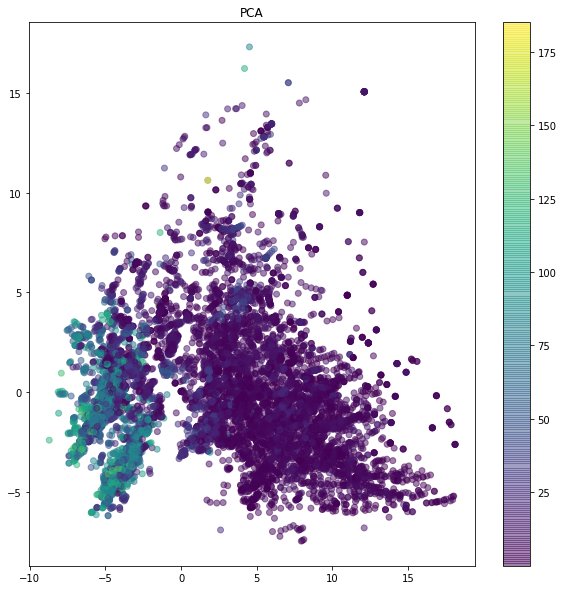
\includegraphics[width=77mm]{img/pca-r.png}}
	\subfigure[]{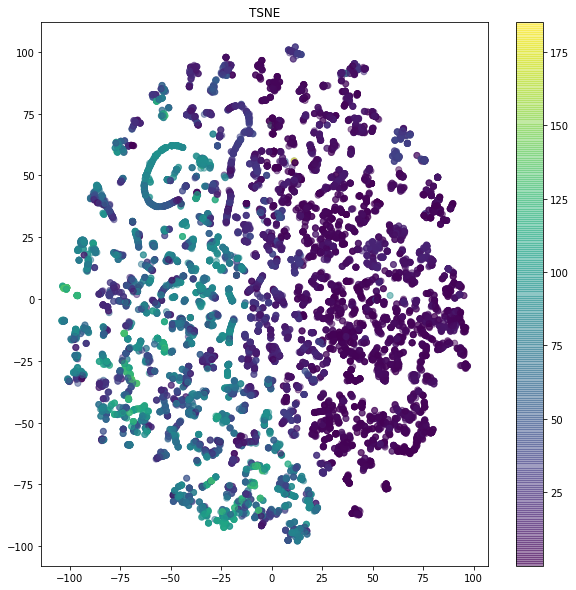
\includegraphics[width=77mm]{img/tsne-r.png}}
	\caption{}
	\label{fig:dimreduction-r}
\end{figure}

Podemos ver que los datos correspondientes a materiales con una temperatura crítica considerablemente diferente no se entremezclan demasiado. Al ser la variable objetivo de tipo continuo, no hay una separación clara entre clases, sino que vemos una transición gradual entre los datos con distinta temperatura crítica. Es decir, hay un punto más o menos definido a partir del cual la tonalidad morada pasa a ser azul, y de azul a verde. 

\subsection{Selección de la clase de funciones a usar}

En este caso nos quedamos con la clase de funciones lineales y con las características lineales originales. No aumentamos la complejidad de la clase añadiendo características cuadráticas o polinómicas de un orden superior, pues esto aumentaría demasiado la dimensionalidad. Dado que disponemos de 81 variables, si añadiéramos características cuadráticas nos quedarían $81^2=6561$ dimensiones, y el aprendizaje conllevaría un tiempo de ejecución bastante alto.  

Por otra parte, la mayor complejidad de la clase haría que aumentara la dimensión de VC, siendo por tanto los modelos más propensos al sobreajuste y habría que incluir una regularización bastante fuerte para paliar este efecto. 

Así pues, optamos por considerar las características originales y entrenar los modelos con las mismas. Además, como veremos en el apartado de preprocesamiento, la mayoría aportan información y no conviene prescindir de ellas. 

\subsection{Hipótesis finales}

Se consideran dos modelos lineales para regresión y se aplica el mismo \textbf{preprocesamiento} a los datos de training y test para los dos modelos. Este consistirá en la normalización de los datos para que todos tengan media 0 y varianza 1, supresión de observaciones anómalas y eliminación de características que aporten poca información al atributo objetivo.

Los dos modelos que se estudiarán serán:
\begin{itemize}
	\item \underline{Support Vector Regression} con Kernel Linear. 
	\item Regresión Lineal con \underline{Modelo Ridge}. 
\end{itemize}

\subsection{Conjuntos de training y test}
Como el conjunto de datos de partida no está dividido en conjuntos para el entrenamiento y test, debemos partirlo antes de empezar con el aprendizaje. Para ello seguimos la regla general de 80\% de los datos para el conjunto de training y el 20\% para test (pues contamos con más de 10000 ejemplos), los cuales se distribuyen de manera aleatoria en los dos subconjuntos. Así nos aseguramos de que ambos subconjuntos pertenecen a la misma distribución y el orden de los datos no es un factor determinante en el aprendizaje. 

Tras realizar la partición, obtenemos un conjunto de training con 17010 datos y con conjunto de test con 4253 ejemplos. 

\subsection{Métrica de error}

La medida de error que usaremos será el error cuadrático medio (MSE,\textit{ mean squared error}): 

$$MSE(w)=\frac{1}{N}\sum_{i=1}^{N}(y_i-w^Tx_i)^2$$

donde N es el número de ejemplos en el conjunto de test, $w$ es el vector de pesos que determina a una función lineal (cuyo error queremos medir) y $(x_i,y_i)$ es el i-ésimo punto de la muestra de test. 

Esta métrica es la más usual en los problemas de regresión. Además, es diferenciable y es la función de pérdida que se usa por defecto en los modelos de regresión. 

Por otra parte, MSE es adecuado para asegurar que nuestro modelo ajustado no tiene predicciones anómalas con errores grandes, pues MSE da más peso a estos errores gracias al cuadrado. Esto es, penaliza bastante los errores grandes. Así, MSE permite tener en cuenta cada uno de los datos individualmente, pues no deja que algún punto tenga un error demasiado alto a cambio de predecir otro con más exactitud (como es el caso de otras métricas como MAE, \textit{mean absolute error})

\underline{Referencias:}

\href{https://towardsdatascience.com/understanding-the-3-most-common-loss-functions-for-machine-learning-regression-23e0ef3e14d3}{https://towardsdatascience.com/understanding-the-3-most-common-loss-functions-for-machine-learning-regression-23e0ef3e14d3}

\subsection{Preprocesamiento}
\subsubsection{Pasos seguidos}
Los pasos llevados a cabo en el preprocesamiento de los datos, tanto de training como de test, han sido los siguientes:
\begin{enumerate}
	\item Normalización de los datos de entrenamiento y test, usando \lstinline|StandardScaler| tal y como hicimos en clasificación, pues SVR trabaja con distancias y es necesario que los datos estén normalizados. De igual forma para la regularización los datos también deben estar normalizados, por lo que ya explicado cuando estudiamos el problema de clasificación. 
	\item  Eliminación de los datos atípicos usando \lstinline|LocalOutlierFactor|, con los mismos parámetros que usamos para clasificación, pues estos dificultan el proceso de aprendizaje y empeoran la solución obtenida, haciendo más propenso el sobreajuste. 
	\item Eliminamos los atributos que aportan poca información haciendo uso en este caso de\\ \lstinline|mutual_info_regression|, que actúa igual que \lstinline|mutual_info_classif| pero estima el valor de MI en el caso de que el atributo objetivo sea una variable continua, como es nuestro caso.
	Así, la función \lstinline|dependence| llamará ahora a \lstinline|mutual_info_regression| en vez de \lstinline|mutual_info_classif|. Nos quedamos con las características que tienen un valor de MI mayor a 0.4. Este umbral puede parecer demasiado alto, pero con este valor sólo se elimina un atributo. De hecho, con un valor de 0.2 también se elimina sólo una variable y con 0.1 ninguna, de modo que todas los atributos aportan bastante información al atributo objetivo y tan sólo uno tiene un valor de MI menor a 0.2.
\end{enumerate}

Cabe destacar que el preprocesamiento ha sido ajustado a los datos de entrenamiento, y no a los de test, a los cuáles sólo se les aplica, de manera que no incurrimos en data snooping. 

Tras llevar a cabo el preprocesamiento nos quedamos con un total de 80 características y 14382 instancias. Así, el número de instancias ha disminuido considerablemente, desde las 17010 que teníamos originalmente en el conjunto de entrenamiento, de modo que se ha eliminado una cantidad considerable de outliers. 

A parte de esos pasos visualizamos la matriz de correlación entre las variables, calculada mediante el coeficiente de correlación de Pearson (función \lstinline|corrcoef|), ya explicado en la parte de clasificación. Dicha matriz es la que sigue: 

\begin{figure}[H]
	\centering
	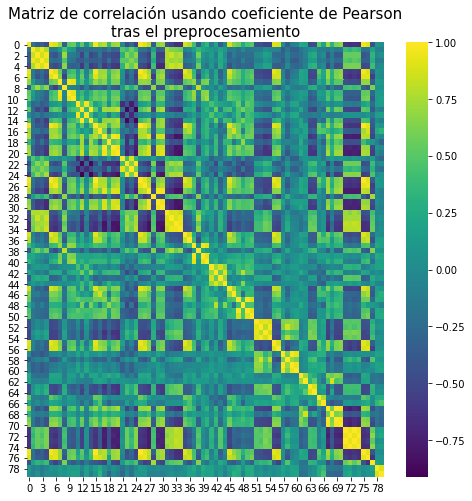
\includegraphics[width=0.6\linewidth]{img/corr2}
	\caption{}
	\label{fig:corr}
\end{figure}

Podemos ver que hay algunas variables con una correlación perfecta, tanto positiva como negativa, pues encontramos algunos puntos amarillos y morados fuera de la diagonal. Sin embargo, en su mayoría la correlación no es muy pronunciada, pues la mayor parte de la matriz es de tonalidad azul-verde. 
\subsubsection{Visualización de los datos preprocesados}

Tras preprocesar los datos los visualizamos en dos dimensiones, de nuevo reduciendo su dimensionalidad con PCA y T-SNE, como venimos haciendo hasta ahora. Los resultados obtenidos han sido:

\begin{figure}[H]
	\centering    
	\subfigure[]{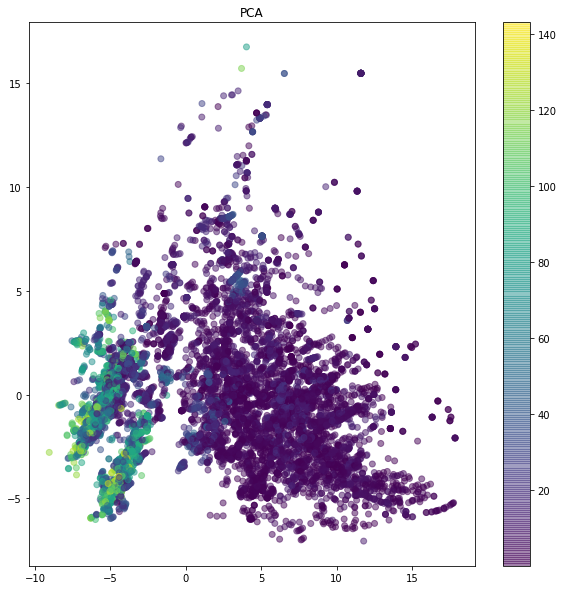
\includegraphics[width=77mm]{img/pca-r2.png}}
	\subfigure[]{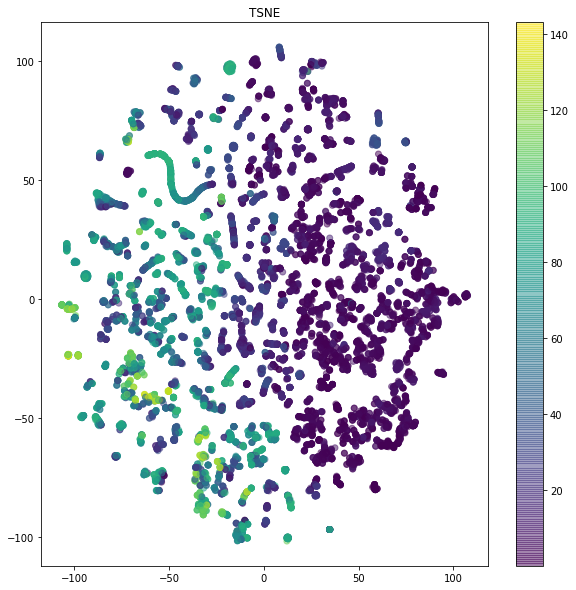
\includegraphics[width=77mm]{img/tsne-r2.png}}
	\caption{}
	\label{fig:dimreduction-r2}
\end{figure}

No podemos extraer demasiadas conclusiones de estas gráficas, pues son muy parecidas a las obtenidas para los datos sin presprocesar. El único aspecto destacable es que ahora los datos con valores de temperatura crítica bastante diferente se entremezclan aún menos, hecho que se aprecia sobre todo en la figura obtenida gracias a T-SNE, pues no hay apenas puntos morados en la zona de los puntos azules y verdes. Esto es debido a la supresión de los outliers. Así, el aprendizaje será más fácil con los datos preprocesados. 

\subsection{Parámetros y regularización}

En un modelo de regresión lineal, la función que se busca minimizar es el error cuadrático medio, que viene dado por la expresión:

$$ E_{in}(w)=\frac{1}{N}\|Xw-Y\|^2$$

donde $N$ es el número de datos de entrenamiento, X es el conjunto de características de los datos de entrenamiento, Y son sus correspondientes etiquetas y w es el vector de pesos que caracterizan a una función lineal, la cual buscamos determinar. 

\subsubsection{Regresión lineal con regularización de tipo Ridge}

El algoritmo de la pseudo-inversa nos da siempre los valores óptimos de los pesos, es decir, determina la función lineal que mejor se ajusta a los datos de entrenamiento, por lo que lo seleccionamos como uno de los modelos a estudiar. Consiste en igualar el gradiente del error cuadrático a 0 y despejar de la fórmula obtenida el vector de pesos w. Esta solución es la óptima para el conjunto de datos de entrenamiento, por lo que proporcionará un valor de $E_{in}=0$. Sin embargo, esto no implica que sea la solución que menor error de generalización tenga, es decir, la de menor $E_{out}=0$, pues es muy probable que se produzca un sobreajuste a los datos de entrenamiento. 

El método de OLS se basa en la independencia entre los atributos. Cuando las variables están correladas y las columnas de  la matriz X tienen una relación aproximadamente lineal, la matriz se acerca a una matriz singular y, en consecuencia, el método de la pseudo-inversa se vuelve muy sensible al ruido en el atributo objetivo, dando lugar a una varianza alta y, por lo tanto, a un mayor error de generalización. 

Como vimos en la Figura 6, hay algunas variables correladas, con un grado alto o medio de correlación, por lo que es necesario incluir regularización. En concreto, como ya comentamos, la regularización de tipo Ridge (o L2) ayuda cuando hay variables correlacionadas. 

No elegimos la regularización de tipo Lasso, pues hemos visto en el preprocesamiento que todas las variables aportan información, por lo que no ayudará al sobreajuste (no pondrá a 0 ningún vector de pesos asociado a una determinada característica).

Así, consideramos un modelo linear regularizado: el modelo Ridge. Este método busca minimizar el error cuadrático medio con un término de penalización añadido, de manera que se restringen los valores que pueden tomar los pesos:

\begin{align*}
\min\limits_{w}\|Xw-Y\|_2^2 + \alpha \|w\|_2^2
\end{align*}

donde $E_{aug}(w)=\|Xw-Y\|_2^2 + \alpha \|w\|_2^2$ es el llamado error aumentado. El gradiente de este error es $$ \nabla_{w} E_{aug}(w)=2X^T(Xw-y)+\alpha w^T$$ que al igualarlo a 0 y despejar el vector de pesos \textbf{w} se obtiene $$w=(X^TX+\alpha I)^{-1}X^Ty,$$ la solución exacta al problema de minimización. 

El parámetro $\alpha$ controla la regularización, esto es, las restricciones a los vectores de  pesos, de modo que cuanto mayor es este valor, más se reducen los pesos y el modelo se vuelve más robusto a la colinealidad de las variables. 

Hacemos uso de \lstinline|sklearn.linear_model.Ridge|, del que ya conocemos algunos de sus parámetros, pues son similares a los de los modelos ya descritos para clasificación: \lstinline|fit_intercept|, que lo dejamos a True, \lstinline|max_iter|, tomamos un máximo de 10000 para que le de tiempo a converger y \lstinline|tol|, que establecemos a 0.0001 para que las solución obtenida sea buena. Además, cuenta con el parámetro de regularización \lstinline|alpha|, cuyo valor tenemos que ajustar mediante una búsqueda en rejilla y validación cruzada. Tenemos también un booleano \lstinline|normalize|, que indica si se quiere que los datos se normalicen con media 0 y varianza 1. Lo dejamos a False puesto que este proceso ya se lleva a cabo en el preprocesamiento. Finalmente, el parámetro \lstinline|solver|, que también conocemos, puede tomar varios valores, entre ellos \textit{sag} y \textit{saga} (que ya comentamos para regresión logística), \textit{svd}, que usa la descomposición en valores singulares de la matriz X para calcular la solución y \textit{cholesky}, que usa la factorización de Cholesky para resolver el sistema de ecuaciones y obtener una expresión cerrada del vector de pesos. Establecemos \lstinline|solver='auto'|, para que se elija automáticamente el solver más adecuado en función de nuestros datos, pues, por ejemplo, no sabemos a priori si la matriz X es definida positiva para poder aplicar la factorización de Cholesky. 
El parámetro \lstinline|random_state| sólo se usa con los solvers sag y saga, para barajar los datos, por lo que lo fijamos por si se seleccionen dichos algoritmos.  

Por lo tanto, el único parámetro que tenemos que configurar de este modelo es el valor de $\alpha$. Para ello utilizamos \lstinline|GridSearchCV| con \lstinline|cv=5| y \lstinline|scoring='neg_mean_squared_error'| (el error cuadrático medio cambiado de signo, que es con el que trabaja sklearn), y le proporcionamos un grid de parámetros con 11 valores entre $10^{-5}$ y $10^5$, para que tenga suficiente margen, como hicimos en el caso de los modelos de clasificación. Así, el mejor valor obtenido ha sido \lstinline|alpha=0.01|.  

 
\underline{Referencias}:

\href{https://scikit-learn.org/stable/modules/linear_model.html#ridge-regression}{https://scikit-learn.org/stable/modules/linear\_model.html}

\href{https://scikit-learn.org/stable/modules/generated/sklearn.linear_model.Ridge.html}{https://scikit-learn.org/stable/modules/generated/sklearn.linear\_model.Ridge.html}

\subsubsection{Support Vector Regression, SVR}

Las máquinas de soporte vectorial, analizadas y explicadas para el caso de clasificación, pueden ser extendidas para resolver problemas de regresión, presentando las mismas ventajas que para clasificación, ya comentadas. 

Al igual que SVM para clasificación, la solución obtenida por SVR sólo depende de los puntos de soporte, y ésta es óptima en el sentido de que minimiza la dimesión de VC. 

SVR ofrece la posibilidad de definir un cierto margen de error $\epsilon$ en el modelo, el cual queda reflejado en las restricciones del problema de optimización como $|y_n-w^Tx_x-b|\leq \epsilon$. Así, cuanto mayor sea el valor de $\epsilon$, más errores se admitirán en la solución obtenida. Por el contrario, si este margen de error es pequeño, se penalizarán casi todos los errores. Así, $\epsilon$ define un margen de tolerancia en el que los errores no se penalizan. Fuera de este margen, un dato $(x_n,y_n)$ se penaliza una cantidad $\xi_n$ ó $ \xi_n^* $, según esté su predicción por encima o por debajo del pasillo determinado por $\epsilon$, respectivamente. 

\begin{figure}[H]
	\centering
	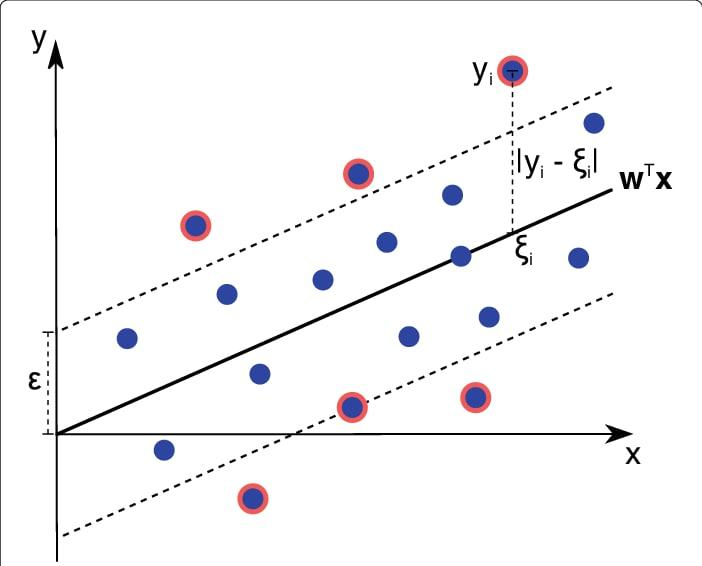
\includegraphics[width=0.6\linewidth]{img/svr}
	\caption{}
	\label{fig:svr}
\end{figure}

Dado un conjunto de instancias $x_n\in\mathbb{R}^d, n=1,2,...,N$ (N es el número de muestras de entrenamiento) y un vector con los valores del atributo objetivo $y\in \mathbb{R}^N$, la formulación primal del problema de optimización a resolver es como sigue: 
\begin{align*}
\min\limits_{b,w,\xi,\xi*}\frac{1}{2}w^Tw + C \sum_{n=1}^{N}(\xi_n+ \xi_n^*)\\
\text{Sujeto a: }  y_n - w^Tx_n - b\leq \epsilon - \xi_n,\\
w^Tx_n + b - y_n  \leq \epsilon - \xi_n^*,\\
\xi_n, \xi_n^* \geq 0 \text{ para } n=1,...,N
\end{align*}



La formulación dual es recomendable cuando el número de características es mayor al número de ejemplos del que se dispone, el cual no es nuestro caso, por lo que usamos el problema primal y no entramos en la descripción del dual. 

Si se usa la función de pérdida \textit{epsilon-intensitive loss}, $e_n(w,b)=max(0,|y_n-(w^Tx_n+b)|-\epsilon)$ para un punto $(x_n,y_n)$, la formulación primal puede escribirse como

\begin{align*}
\min\limits_{b,w}\frac{1}{2}w^Tw + C \sum_{n=1}^{N}max(0,|y_n-(w^Tx_n+b)|-\epsilon)
\end{align*}

Con esta función de pérdida los errores menores a $\epsilon$ son ignorados. 

que es el problema de optimización que resuelve \lstinline|LinearSVR|, modelo que vamos a usar. 

El parámetro C determina el efecto de la penalización por salirse del pasillo, es decir, cuánto afectan los valores de $\xi_n$ y $ \xi_n^* $, y equivale a la inversa del parámetro de regularización $\alpha$, que vimos en el modelo de Ridge. Así, cuando mayor sea $C$, más peso tienen las penalizaciones $\xi_n$ y $ \xi_n^* $ por salirse del pasillo, y menos influencia tendrá la regularización, y viceversa. 

Como ya comentamos para el caso de \lstinline|LinearSVC|, el solver usado por estos modelos es liblinear. 

Describimos ahora los parámetros que acepta \lstinline|LinearSVR|. Muchos de ellos son los que ya conocemos, y consideramos los mismos valores que les hemos dado hasta ahora, por los motivos que se han ido explicando: \lstinline|fit_intercept=True|, \lstinline|intercept_scaling=1|, \lstinline|dual=False|, \lstinline|max_iter=10000| y \lstinline|tol=0.0001|. El parámetro de regularización \lstinline|C| y el margen de error \lstinline|epsilon| los ajustaremos mediante una búsqueda en rejilla y validación cruzada. Como función de pérdida \lstinline|loss| tomamos \lstinline|squared_epsilon_insensitive|, que es el cuadrado de la función \textit{epsilon-intensitive}, por ser diferenciable y penalizar los errores grandes, como ya hemos comentado para otras funciones de pérdida que usan la norma 2. El parámetro \lstinline|random_state| se usa para fijar la semilla para barajar los datos.  

Como venimos haciendo hasta ahora para configurar los valores de los parámetros usamos \lstinline|GridSearchCV| con \lstinline|cv=5| y \lstinline|scoring='neg_mean_squared_error'|. Para el parámetro epsilon tomamos 6 valores entre $10^{-6}$ y $0.1$, y obtenemos como mejor valor $\epsilon=0.000001 $. Para C consideramos, como siempre, 11 valores entre $10^{-5}$ y $10^5$ y obtenemos que el mejor de ellos es $C=10000$. 

\underline{Referencias:} 

\href{https://scikit-learn.org/stable/modules/svm.html#mathematical-formulation}{https://scikit-learn.org/stable/modules/svm.html}

\href{https://towardsdatascience.com/an-introduction-to-support-vector-regression-svr-a3ebc1672c2}{https://towardsdatascience.com/an-introduction-to-support-vector-regression-svr-a3ebc1672c2}

\href{https://scikit-learn.org/stable/modules/generated/sklearn.svm.LinearSVR.html#sklearn.svm.LinearSVR}{https://scikit-learn.org/stable/modules/generated/sklearn.svm.LinearSVR.html}

\subsubsection{Análisis de los mejores valores de los hiperparámetros}

Hemos visto que para los dos modelos analizados se obtienen valores bajos del parámetro de regularización: para Ridge obtuvimos $\alpha=0.01$ y para SVR $C=10000$, que equivale a $\alpha=0.00001$. Esto indica que la regularización tiene poco efecto en nuestros modelos. Además, en el caso de SRV el mejor valor para el margen de error era aquel que consideraba un margen muy pequeño, $\epsilon=10^{-5}$, casi inapreciable, de manera que si no se toleran los errores la solución obtenida es mejor. 

Este hecho puede ser debido a la simplicidad de nuestra clase de funciones, pues solo consideramos características lineales y disponemos únicamente de 80 características. La varianza de la clase (y por tanto el error determinístico) es pequeña, de modo que el sobreajuste no supone un grave problema. 

La matriz de correlaciones, representada en la Figura 6, no muestra demasiadas características con correlación lineal perfecta, por lo que la mayoría de ellas son importantes para el aprendizaje y el vector de pesos asociado a cada una de ellas no tiene por qué ser reducido, de ahí que la regularización de tipoo Ridge no afecte. 

\textbf{Nota:} Al igual que para el problema de clasificación consideramos la variable \lstinline|TUNING|, para determinar si se ejecuta o no el grid de parámetros. Por defecto la ponemos a False, pero para este problema, al contrario que el anterior, el tiempo de ejecución es relativamente bajo, por lo que puede cambiarse a True sin problema para comprobar los resultados. 

\subsection{Selección de la mejor hipótesis}

Para seleccionar el mejor de los dos modelos estudiados usaremos validación cruzada con 5 particiones, tal y como hicimos para el problema de clasificación, y por los motivos allí explicados. En esta ocasión nos quedaremos con aquella hipótesis que presente el menor error cuadrático medio de validación cruzada. 

Utilizamos la función \lstinline|cross_val_score| dentro de \lstinline|printCV|, y llamamos a esta última con nuestros dos modelos con sus parámetros ajustados. El comportamiento de estas dos funciones ya se explicó en el problema de clasificación. La única diferencia es que ahora se usa MSE como métrica en lugar del \textit{accuracy}. Los resultados obtenidos han sido los siguientes: 

\begin{lstlisting}
Ridge: 291.08466633522585
Support Vector Regression: 291.0803893185365
\end{lstlisting}

Ambos errores son bastante altos, lo cual puede ser consecuencia de la simplicidad de la clase de funciones elegida, que es posible que no sea capaz de explicar toda la variabilidad de los datos. En este caso estaríamos ante un problema de underfitting. Además, los modelos elegidos son lineales y simples, lo cual influye aún más en la poca calidad de las soluciones obtenidas. 

Nos damos cuenta también de que los errores son prácticamente iguales, por lo que podríamos decir que los dos modelos considerados presentan la misma bondad en este problema. 

Sin embargo, siguiendo el criterio de elegir el que tiene menor error de validación cruzada, nos quedamos con SVR, que ofrece un error ligeramente inferior. Así pues, llamamos a la función \lstinline|printFinalResult| con SVR para que nos muestre los errores sobre el conjunto de entrenamiento y test obtenidos por este modelo. En este caso la métrica que usa dicha función es MSE. 

\begin{lstlisting}
Error en el conjunto de entrenamiento:  288.01810499725843
Error en el conjunto de test:  306.7099998917412
\end{lstlisting}

El error en el conjunto de test es bastante elevado, mayor que el de validación cruzada, lo cual era de esperar pues los datos de test nunca han sido vistos por el modelo. La diferencia entre el error de validación y el de test es de más de 16, aunque teniendo en cuenta cómo de elevados son los errores esta diferencia no es demasiado significativa. 

Por otra parte, el error en el conjunto de entrenamiento también es considerablemente grande, de modo que nuestra clase de funciones no es capaz de ajustarse a la muestra y el error no es debido a sobreajuste, sino todo lo contrario. Así, podemos afirmar que hay underfitting. Por este motivo la regularización no tenía efecto, pues lo que hay que hacer es aumentar aún más la complejidad de la clase y no restringirla, que es lo que hace la regularización. 

Tenemos que $E_{out}\approx E_{test}=307.11899832417$. 

\subsection{Entrenamiento con todos los datos }

Para intentar mejorar la solución encontrada por el mejor modelo vamos a entrenarlo con todos los datos juntos, tanto de training como de test. 

Para ello procedemos de la misma forma que hicimos en el problema de clasificación en este punto: unimos todos los datos originales en un único conjunto, los barajamos y le aplicamos el preprocesamiento al nuevo conjunto obtenido. Obtenemos así 17642 instancias y 80 características. 

Calculamos el error de validación cruzada, llamando a \lstinline|printCV| con SVR con sus mejores parámetros y con el nuevo conjunto de datos. Obtenemos que $E_{cv}=289.4529681762297$, algo menor que el error de validación cruzada que conseguimos cuando usamos sólo el conjunto de datos de entrenamiento, y también menor que el error en el conjunto de test. 

Se cumple que $$E_{out}\leq E_{cv}=289.453$$ y antes $E_{out}\approx E_{test}=307.11$, de manera que el error fuera de la muestra disminuye al entrenar con más datos, lo cual era de esperar. 

\end{document}